\section{Definition der Anwendung} \label{Anwendungsdefinition}
	Als Anwendung für den Versuchsaufbau wurde die Verbindung zweier Platten über einen Befestigungswinkel definiert. Die Platten bestehen aus Kunststoff und sind mit drei Befestigungslöcher, wie auch Fingerzinken versehen. Der Prozess wird durch 3 Teilprozesse gebildet. 
	\vspace{3mm}
	
	\textbf{Teilprozess 1:} Positionieren der Platten
	\vspace{2mm} 
	\\
	 Der Teilprozess fügt die beiden Platten im 90°-Winkel zusammen (\ref{fig:Teilprozess 1}). Die Seiten der Platten sind mit Fingerzinken versehen, die ineinandergreifen. Der Roboter entnimmt zunächst die erste Platte aus dem Lager und positioniert sie auf einer Halterung. Anschliessend holt der Roboter die zweite Platte und stosst diese entsprechend der Fingerzinken in die erste Platte.
	 \vspace{3mm} 
	 
	 \textbf{Teilprozess 2:} Montieren von Befestigungswinkel 
	 \vspace{2mm}
	 \\
	 Der Roboter holt den Befestigungswinkel aus dem Lager und platziert diesen entsprechend der Löcher in den Platten (\ref{fig:Teilprozess 2}). Die korrekte Position wird über ein Vision-System definiert. Das Befestigungsblech kann auch in die Halterung eingelegt werden.
	 \vspace{3mm}
	 
	 \textbf{Teilprozess 3:} Verbinden von Platten mit Befestigungswinkel 
	 \vspace{2mm} 
	 \\
	 Im letzten Schritt werden die Befestigungswinkel via Stifte mit den Platten verbunden (\ref{fig:Teilprozess 3}). Die Passung der Löcher ist dabei so ausgelegt, dass der Stift knapp mit Spiel montiert werden kann. Die Stifte müssen somit so mit der Platte verbunden werden, dass sich diese nicht verkanten. 
	 \vspace{3mm}
	 
	 \begin{figure}[h!]
	 	\centering
	 	\begin{subfigure}[b]{0.28\textwidth}
	 		\centering
	 		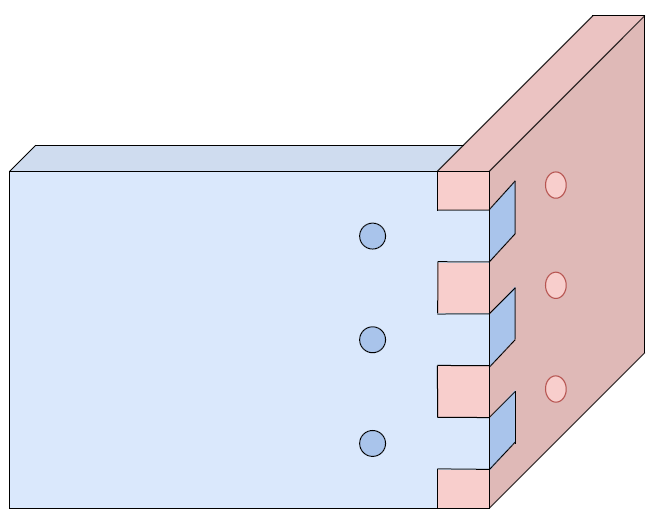
\includegraphics[width=\textwidth]{04_Anwendung_und_Aufbau/Teilprozess_1}
	 		\caption{Teilprozess 1}
	 		\label{fig:Teilprozess 1}
	 	\end{subfigure}
	 	\hfill
	 	\begin{subfigure}[b]{0.28\textwidth}
	 		\centering
	 		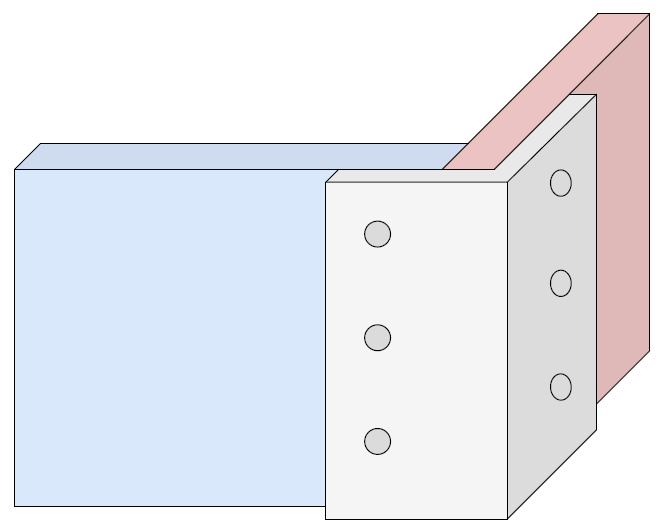
\includegraphics[width=\textwidth]{04_Anwendung_und_Aufbau/Teilprozess_2}
	 		\caption{Teilprozess 2}
	 		\label{fig:Teilprozess 2}
	 	\end{subfigure}
	 	\hfill
	 	\begin{subfigure}[b]{0.32\textwidth}
	 		\centering
	 		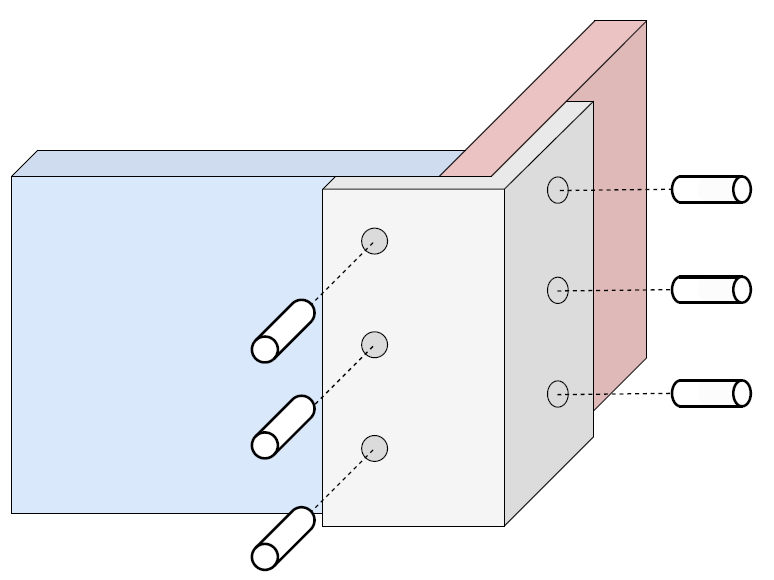
\includegraphics[width=\textwidth]{04_Anwendung_und_Aufbau/Teilprozess_3}
	 		\caption{Teilprozess 3}
	 		\label{fig:Teilprozess 3}
	 	\end{subfigure}
	 	\caption{Anwendungsteilprozesse}
	 	\label{fig:Teilprozesse}
	 \end{figure}
	 
	
	 \newpage
	 